\chapter{Metodología}
\label{chap:metodologia}

\lettrine{E}{n} este capítulo se expondrá la metodología elegida. En nuestro caso, optamos por una metodología incremental ágil con una gestión del flujo de trabajo mediante Kanban.

\section{Introducción a la metodología}

Para este proyecto se termino optando por la metodología ágil \cite{scrum}. En concreto, se optó por un enfoque basado en un desarrollo incremental, donde la gestión del flujo de trabajo se realizó con Kanban.


Este enfoque incremental permite desarrollar pequeños incrementos que van mejorando y puliendo las funcionalidades de nuestro sistema de forma progresiva. Esta metodología se adapta muy a entornos donde los requisitos no están de todo claros en el principio y en el futuro son susceptibles a cambios. Este es el caso de un trabajo de fin de grado donde normalmente se empieza con una idea pero no se sabe muy bien como abordar el problema desde un principio, por lo que tener esta flexibilidad para hacer cambios conforme avance el proyecto y recibamos retroalimentación es muy útil. 

La Gestión de Flujo de Trabajo Kanban se implementó empleando un tablero visual en la plataforma Notion. Esta metodología facilitó una gestión eficiente del flujo de trabajo al proporcionar una representación visual de las tareas, organizadas en categorías de pendientes, en progreso y completadas. Además es muy fácil realizar ajustes en estas tareas según la retroalimentación recibida en las reuniones.


\begin{figure}[h]
\centering
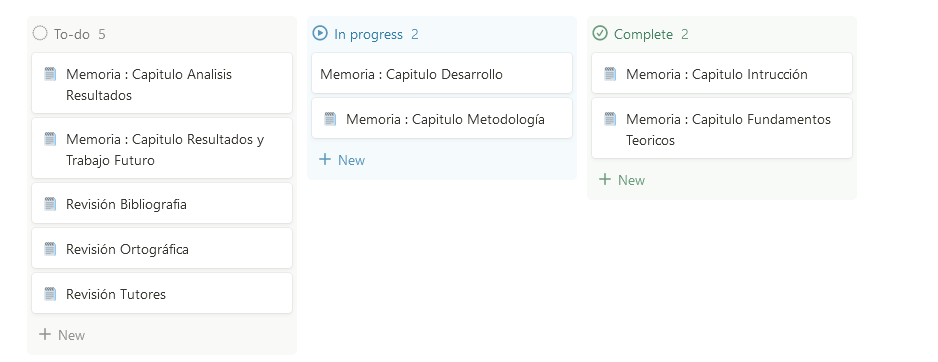
\includegraphics[width=14cm]{imaxes/kanban.png}
\label{fig:pointnetc}
\caption{Ejemplo de Kanban para el desarrollo de la memoria}
\end{figure}


\section{Desarrollo Incremental}

Previamente se introdujo el desarrollo incremental, ahora lo comentaremos con más detalle.
Este desarrollo se basa en la premisa de que es más efectivo y adaptable desarrollar algo en partes pequeñas y simples en vez de abordar el proyecto en su totalidad de una sola vez. Cada incremento se desarrolla en un período de tiempo determinado con un grupo de funcionalidades. Esto nos permite obtener retroalimentación temprana para saber si nos estamos desviando y ajustarnos al resultado que buscamos. Además, al desarrollar en partes pequeñas se reduce el riesgo de desarrollar algo incorrecto y darnos cuenta al final.

\subsection{Incrementos}

Los incrementos son unidades de trabajo que representan un conjunto de funcionalidades entregables. Cada incremento agrega nuevas funcionalidades o corrige las anteriores, y está diseñado para ser funcional por sí mismo. Al final de cada incremento, en nuestro caso, era revisado con los tutores del trabajo, y se discutían las futuras líneas de trabajo sobre él, así como la forma en que podríamos mejorar lo hecho hasta ahora.


\begin{figure}[h]
\centering
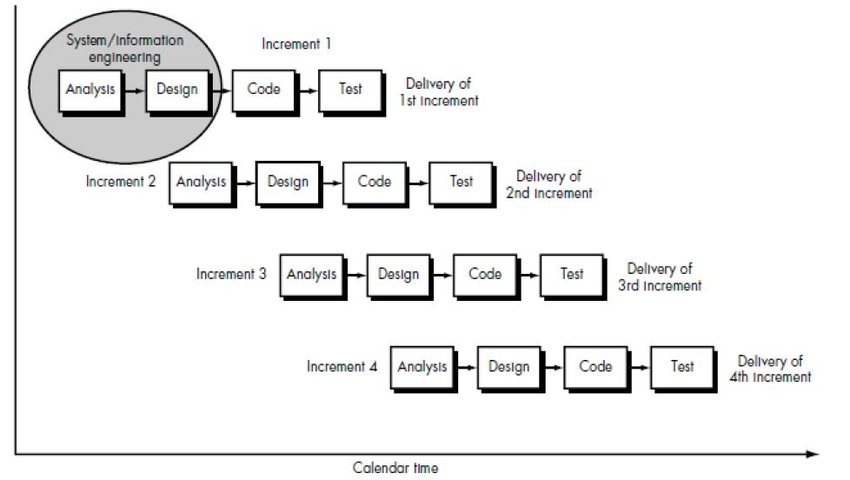
\includegraphics[width=12cm]{imaxes/Incremental-software-development-model.png}
\label{fig:pointnetc}
\caption{Ejemplo de un desarrollo incremental \cite{inproceedings}}
\end{figure}


